\documentclass{beamer}
\usepackage{hyperref}
\usepackage{listings}

\usepackage{color}
\usepackage{setspace}


\definecolor{Code}{rgb}{0,0,0}
\definecolor{Decorators}{rgb}{0.5,0.5,0.5}
\definecolor{Numbers}{rgb}{0.5,0,0}
\definecolor{MatchingBrackets}{rgb}{0.25,0.5,0.5}
\definecolor{Keywords}{rgb}{0,0,1}
\definecolor{self}{rgb}{0,0,0}
\definecolor{Strings}{rgb}{0,0.63,0}
\definecolor{Comments}{rgb}{0,0.63,1}
\definecolor{Backquotes}{rgb}{0,0,0}
\definecolor{Classname}{rgb}{0,0,0}
\definecolor{FunctionName}{rgb}{0,0,0}
\definecolor{Operators}{rgb}{0,0,0}
\definecolor{Background}{rgb}{0.98,0.98,0.98}

\lstset{
numbers=left,
numberstyle=\footnotesize,
numbersep=1em,
xleftmargin=1em,
framextopmargin=2em,
framexbottommargin=2em,
showspaces=false,
showtabs=false,
showstringspaces=false,
frame=l,
tabsize=4,
% Basic
basicstyle=\ttfamily\small\setstretch{1},
backgroundcolor=\color{Background},
language=Python,
% Comments
commentstyle=\color{Comments}\slshape,
% Strings
stringstyle=\color{Strings},
morecomment=[s][\color{Strings}]{"""}{"""},
morecomment=[s][\color{Strings}]{'''}{'''},
% keywords
morekeywords={import,from,class,def,for,while,if,is,in,elif,else,not,and,or,print,break,continue,return,True,False,None,access,as,,del,except,exec,finally,global,import,lambda,pass,print,raise,try,assert},
keywordstyle={\color{Keywords}\bfseries},
% additional keywords
morekeywords={[2]@invariant},
keywordstyle={[2]\color{Decorators}\slshape},
emph={self},
emphstyle={\color{self}\slshape},
%
}


\title{Cassandra, Hadoop, Pig}
\subtitle{Apache}
\author{Konrad Kurdej}
\date{30-07-2013}
\usetheme{Hannover}

\AtBeginSection[] { 
  \begin{frame}[plain] 
    \tableofcontents[currentsection] 
  \end{frame}
  \addtocounter{framenumber}{-1} 
}


\begin{document}
\begin{frame}
\titlepage
\end{frame}
\section*{Outline}
\begin{frame}
\tableofcontents
\end{frame}

\section{Cassandra}

\begin{frame}
    \begin{itemize}
        \item implementation of Google's BigTable and Amazon's Dynamo
        \item developed at Facebook
        \item NoSQL - key-value store mixed with columns
        \item no joins or subqueries, emphasizes denormalization
        \item has data structures - list, set, map (64kb limit) - and counters
        \item focused on writes but reads are also fast
    \end{itemize}

\end{frame}


\begin{frame}
\begin{itemize}
 \item used by: Netflix, eBay, Twitter, Reddit, ...
 \item fault tolerant - no single point of failure, replication
 \item performant
 \item decentralized
 \item durable
 \item configurable (for example: (a)sync replication)
 \item scalable \href{http://vldb.org/pvldb/vol5/p1724_tilmannrabl_vldb2012.pdf}{PAPER}
 \item there are companies that provide support
\end{itemize}
\end{frame}


\begin{frame}
    \frametitle{CQL 3 \& Data modeling}
%\href{http://www.datastax.com/documentation/cassandra/1.2/index.html?pagename=docs\&version=1.2\&file=index#cassandra/ddl/ddl_anatomy_table_c.html#concept_ds_qqw_1dy_zj}{example from documentation}
\end{frame}


\begin{frame}
    \frametitle{Sad part}
    \begin{itemize}
        \item you can't do much in CQL 3
            \pause
        \begin{itemize}
            \item ... WHERE COL1 != COL 2;
                \pause
            \item UPDATE on all rows
                \pause
            \item arithmetic in UPDATE is limited to add/sub on counters
        \end{itemize}
            \pause
        \item support ? echo ... echo ... echo ...
            \pause
        \item never paste stacktrace on IRC
            \pause
        \item JIRA - closed ticket - we don't care
            \pause
        \item branch 1.2.x, x+1 about every 4 weeks, 1.2.7 on Friday, on Sunday we have 1.2.8
            \pause
        \item "InvalidRequestException(why:Expected 8 or 0 byte long (4))"
    \end{itemize}
\end{frame}


\section{Hadoop}

\begin{frame}
    \begin{block}{Open-source software for reliable, scalable, distributed computing}
        Modules:
        \begin{description}
            \item[Common] utilities supporting other modules
            \item[HDFS] high-throughput distributed file system
            \item[YARN] framework for job scheduling and resource management
            \item[MapReduce] YARN-based system for parallel processing of large data sets
        \end{description}
    \end{block}
\end{frame}



\begin{frame}
    \frametitle{MapReduce - patent 7,650,331}
    Sounds functional. \pause Isn't that much.
    \begin{block}{map}
        $ map: K \times V \rightarrow list (K' \times V') $
    \end{block}
    \begin{block}{reduce}
        $ reduce: K' \times list(V') \rightarrow list (V'')$
    \end{block}

    Map output is sorted and grouped by keys to make proper input into reducers.

    \begin{itemize}
        \item very popular paradigm. Avalible even in MongoDB.
        \item good for big batch jobs
        \item requires distributed input/output, like Cassandra
        \item big latency is serious drawback making it useles in real-time applications
    \end{itemize}

\end{frame}



\begin{frame}
    \begin{itemize}
        \item Hadoop world is dominated by Java
            \pause
        \item but they are not blind - Hadoop Streaming - any language - stdin/stdout
        \item some libs simulate MR without Hadoop
        \item others wrap it Hadoop Streaming - mrjob
        \item streaming still doesn't free us if we would like to provide our input/output
    \end{itemize}
    \begin{block}{mrjob}
    Python library. Runs localy, on hadoop or Amazon Elastic MapReduce.
    \end{block}
\end{frame}


\begin{frame}
    \lstinputlisting[language=Python]{mrjob_wc.py}
\end{frame}


\section{Pig}



\begin{frame}
\begin{center}


\includegraphics[scale=0.5]{BUGSBUGSEVERYWHERE.jpg} 

\end{center}

\end{frame}


\begin{frame}
\begin{center}
\Huge{Q \& m A}

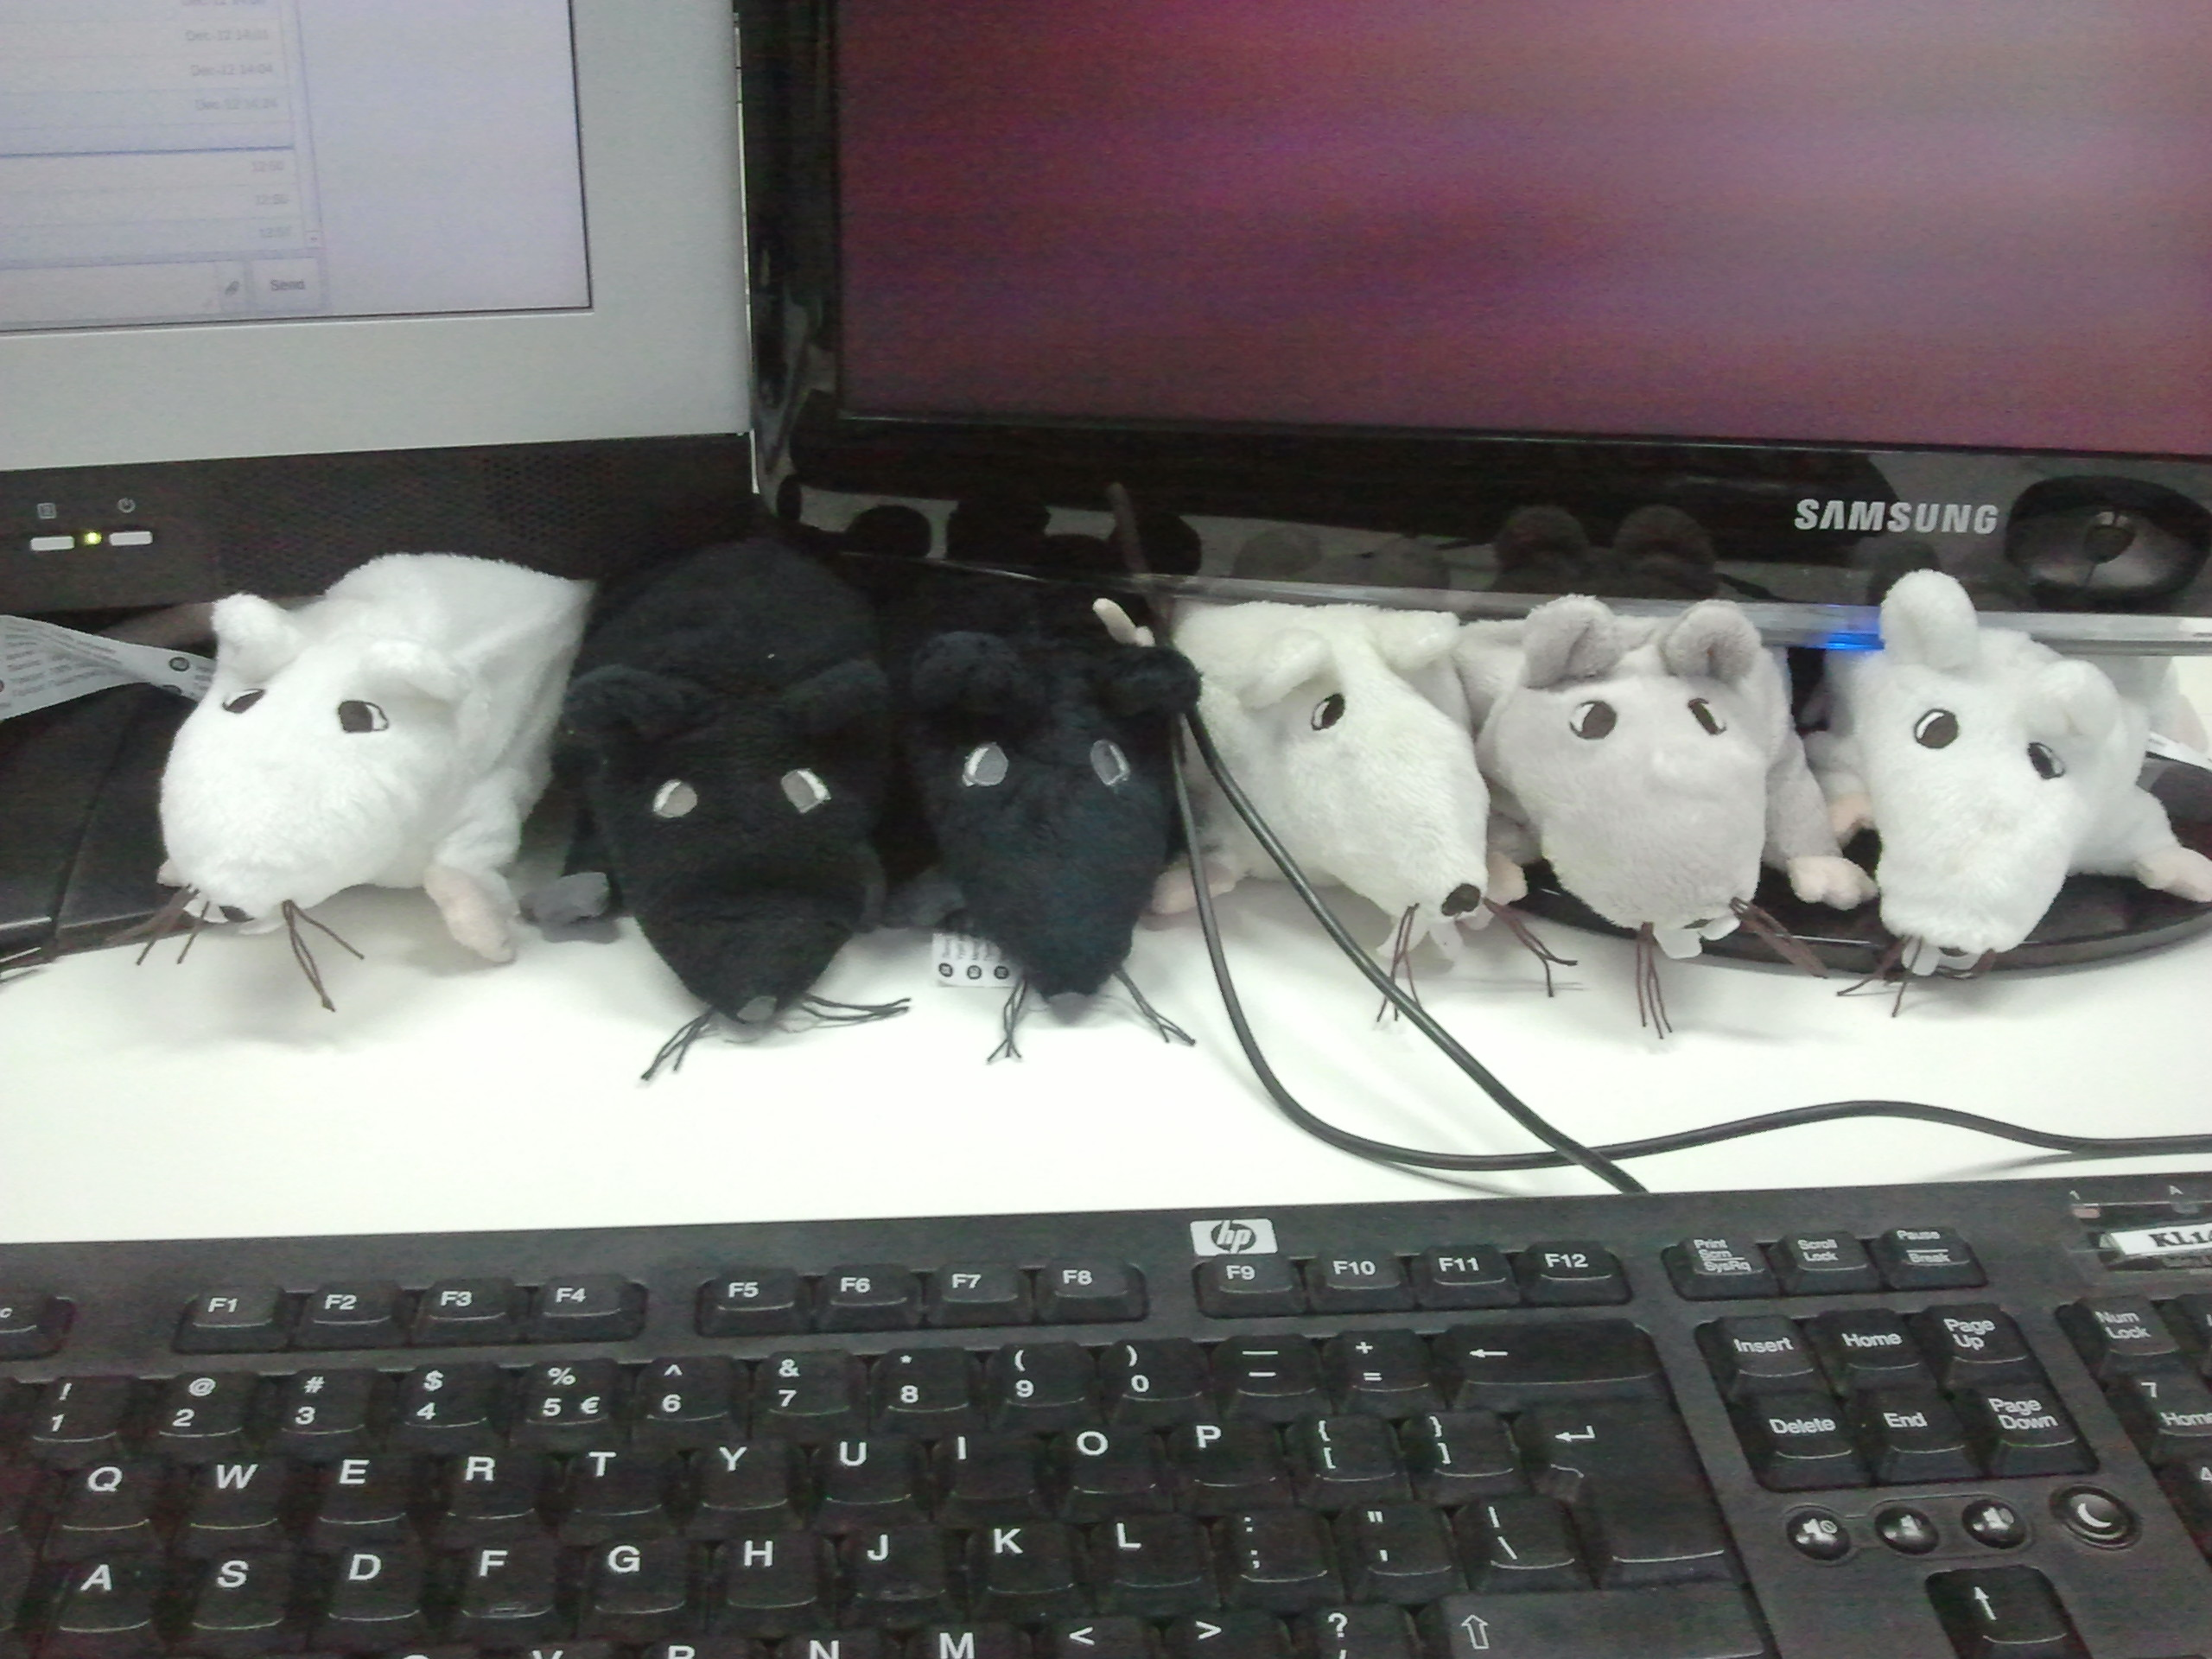
\includegraphics[scale=0.1]{../common/questions.jpg} 

\end{center}

\end{frame}

\end{document}
